\chapter{Design}

\section{Architecture}

The designed architecture of the project can be observed in the figure \ref{fig:arch}. There are three data sources connected to Grafana through an extended version of the official SimpleJson data source plugin. Each data source access the data it provides in different ways; through an outside service, from a database or from memory.

\begin{figure}[h]
	\centering
	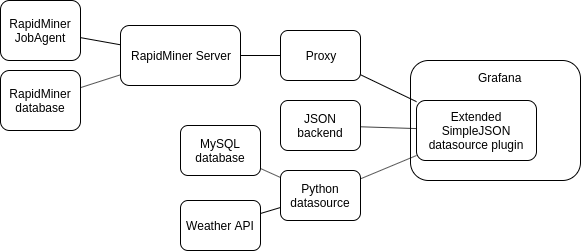
\includegraphics[width=150mm, keepaspectratio]{figures/architecture.png}
	\caption{Architecture diagram}
	\label{fig:arch}
\end{figure}

%---
\section{Components}
%---

In this section, each component is presented, focusing on their responsibilities.

%---
\subsection{Extended SimpleJSON datasource plugin}
%---

Grafana uses data source plugins to connect to different data storage backends. These components usually poll their backends, sending query requests to acquire the recorded information. Each data source plugin exposes a Grafana specific interface which allows Grafana to communicate with each data source plugin the same way.

% https://github.com/grafana/simple-json-datasource
The SimpleJSON datasource is made by the Grafana team and is available on GitHub (insert reference HERE).

It has two main purposes. One is to act as an example implementation to make writing custom data source plugins easier for the community. The other is to enable Grafana to read data from services that expose data in JSON format (which is widely popular thorough the industry).

For this thesis project, the latter role seems to be more important, as it possible to create a tool that receives data from different kind of formats and translates them into JSON. This way, we can send the transformed data to Grafana, which as a result would be able to display the collected data in one place that originally came from various sources.

Hence, instead of designing a data source plugin for Grafana from scratch, I chose to customize this already available component to dodge many caveats of developing an own plugin for a complex system.

% https://github.com/grafana/simple-json-datasource/blob/master/README.md
The SimpleJSON data source plugin requires its backend to implement the following endpoints:

\begin{itemize}
	\item \emph{/} - This endpoint is used for testing the connection between Grafana and the data backend. If everything is in order on the side of the backend, this endpoint should a HTTP 200 response.
	\item \emph{/search} - This endpoint is used for finding the available metric options. For example the names for different time-series.
	\item \emph{/query} - This endpoints is used to acquire the actual metrics data from the backend.
	\item \emph{/annotations} - This endpoint is used to return objects called annotations, additional information attached to metrics data. In the context of this project, we do not use this feature, however, it is needed for the data source plugin to run without errors.
\end{itemize}

In order to introduce additional interactivity capabilities, when integrating the RapidMiner Webservice, the SimpleJSON data source plugin needs to be extended. Since it is possible for a RapidMiner Webservice to accept parameters, which can filter the result, it would be useful to be able to acquire these available exposed parameters, so we can make more accurate metric queries with Grafana.

This means that the plugin has to be able to send another type of request to the backend, which in return would respond with the list of the accessible parameters:

\begin{itemize}
	\item \emph{/parameters} - This endpoint is used for acquiring the available query parameters exposed by the backend.
\end{itemize}

\begin{center}
	--- TODO ---
	\begin{itemize}
		\item extended API for SimpleJSON datasource
		\subitem querying available paramaters for a RM webservice
		\item explain how the datasource communicates with the backend
		\item show the requested/returned data formats? -> rather implementation
	\end{itemize}
\end{center}


%---
\subsection{Proxy}
%---

The main responsibility of this component is to translate between the RapidMiner Web service which the RapidMiner Server exposes and the SimpleJSON datasource plugin. The problem is that RapidMiner Server exposes its result in JSON, but is in another format that the SimpleJSON data source plugin accepts.

To accomplish that this proxy component could communicate with Grafana, it must implement the endpoints required by the SimpleJSON plugin. These were explained in the section describing the plugin.

So the gateway component should be able to handle HTTP requests from SimpleJSON as well as forwarding them to RapidMiner after the translation. For this reason, it must be a constantly available service.

There are some RapidMiner web service specific considerations which need to be taken into account while designing the gateway component. We have to define the actions made by the proxy towards the RapidMiner Server in an abstract way, in order to properly implement the component.

When accepting requests on the \texttt{/search} endpoint the gateway should return with the names of the available RapidMiner web services in a format that the data source plugin accepts. For that, it must send a request to the RapidMiner Server, asking for these names each time, so it is ensured that the information is always up-to-date. This is crucial, as the name of the RapidMiner web service determines the address where the gateway has to send the query requests later.

The \texttt{/parameters} endpoint should return the parameters exposed by the given web services. This information also falls in the category that should not be cached, as the possession of false knowledge can lead to failed queries that ends in no data displayed in Grafana.

After we have the name of the web service and its available parameters, we can finally request the actual data. For that, we use the \texttt{/query} endpoint. This is the place when the translation of different different data formats happens.

%---
\subsection{JSON backend}
%---
% https://github.com/bergquist/fake-simple-json-datasource
This component is a example backend implementation for the SimpleJSON data source plugin. It serves as a base for creating other backends for the data source plugin. It also further expresses the general usability of the SimpleJSON plugin.

%---
\subsection{Python data source}
%---

Similarly as the Proxy component, the Python data source also needs to have those endpoints required by the SimpleJSON data source plugin, so this part is analogous to that in the Proxy. The effects of invoking them are slightly different than in case of the Proxy, because this Python source uses two components as backends, an 'external' API service and a separate database as described in section \ref{case-study-python-source}.


\begin{center}
	--- TODO ---
\end{center}


%---
\subsection{Weather API}
%---

This component represents the previously mentioned external service. Its responsibility is to expose a service that can be utilized by other softwares in order to acquire additional business-relevant information.

%---
\subsection{MySQL database}
%---

The Python datasource uses this database component to read some sample data from it.


%\begin{itemize}
%	\item why do we need a gateway
%	\item how can we access data from RapidMiner WebService
%	\item why is it good to have a python compoment between Grafana and MySQL
%	\begin{itemize}
%		\item we can customize it better, what we see from the database
%		\item can implement business logic, only see business-relevant projections, granularity of the data
%		\item can aggregate data from different backends
%		\item can aggregate data with outsider APIs (POC implementation for this use-case)
%	\end{itemize}
%\end{itemize}


\begin{itemize}
	\item Grafana
	\item proxy/gateway
	\item python-datasource
	\begin{itemize}
		\item python-datasource
		\item mysql
		\item weather-api
	\end{itemize}
	\item RapidMiner stack
	\begin{itemize}
		\item rapidminer-server
		\item job-agent
		\item database
	\end{itemize}
	\item Grafana datasource plugin (extended API - parameters)
	\begin{itemize}
		\item extended API for asking for available parameters
		\item extended GUI, that dynamically lists available parameters (specify SOURCE!!!!!!!)
	\end{itemize}
	\item Grafana extended panel plugin
\end{itemize}